\section{CU4 - Utilisation comme plateforme de TPs}

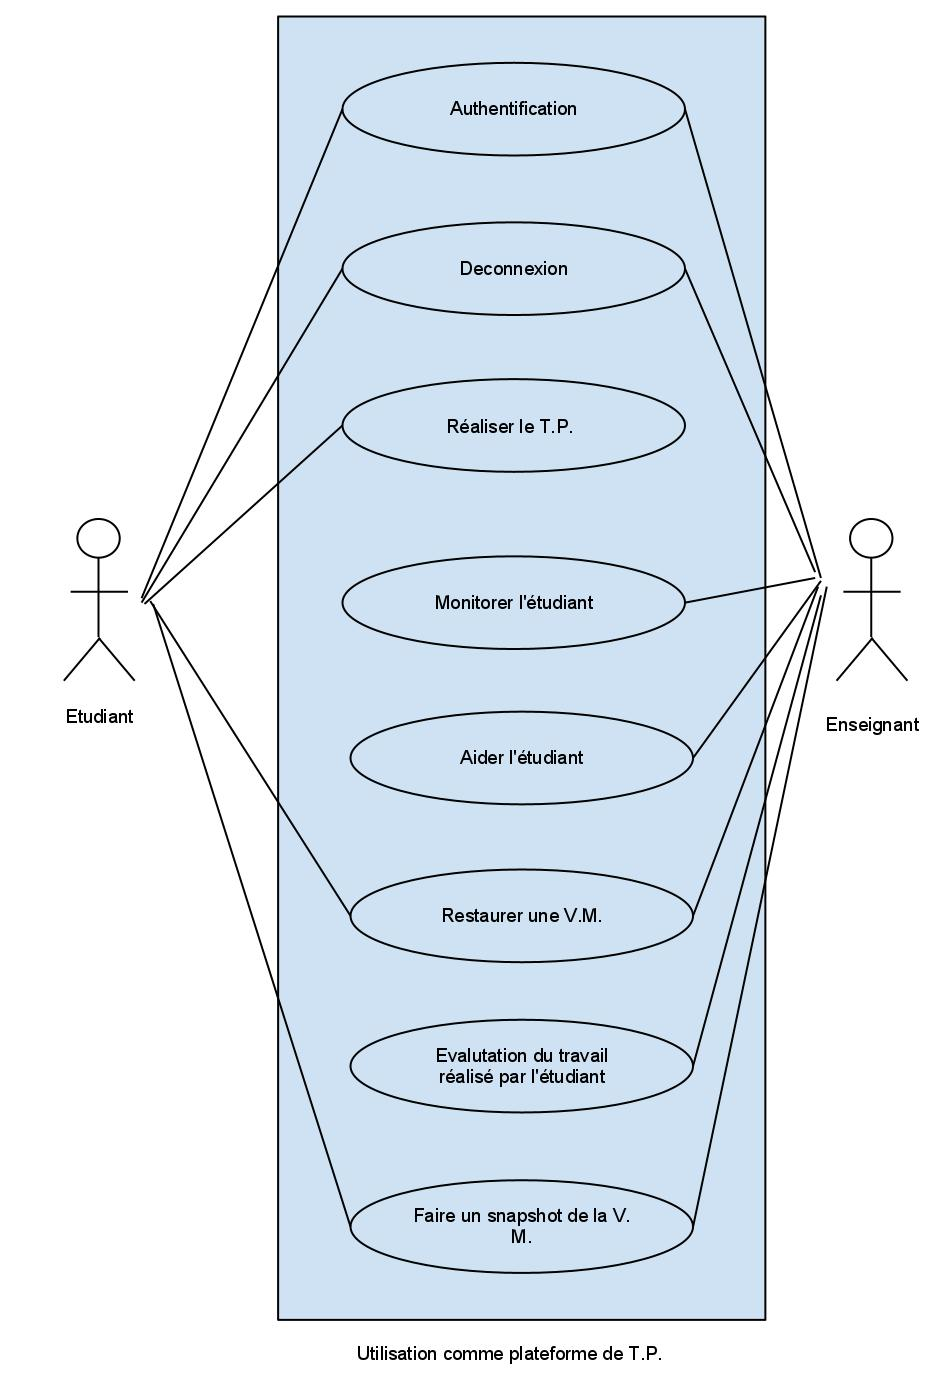
\includegraphics[scale=0.4]{CU4.jpg}

L’un des objectifs pédagogiques de la solution est de pouvoir réaliser des plateformes de T.P. axées autour de l’utilisation des machines virtuelles.

L’étudiant (et l’enseignant) doit tout d’abord se connecter (\underline{authentification}) pour pouvoir utiliser la machine virtuelle du T.P.
L’étudiant réalise ensuite le travail demandé pour le T.P. (\underline{réaliser le T.P.}). Pendant ce temps, l’enseignant a la possibilité de \underline{monitorer l’étudiant}, et de l’aider si besoin (\underline{aider l’étudiant}).

L’étudiant (ainsi que l’enseignant) a la possibilité \underline{faire un snapshot de la V.M.}, et d’effectuer un backup de l’état de la machine (\underline{restaurer une V.M.}).

L’enseignant pourra ensuite \underline{évaluer le travail de l’étudiant}.

Enfin, l’étudiant (ainsi que l’enseignant) devra \underline{se déconnecter} de la machine virtuelle.